\documentclass[aspectratio=169]{../latex_main/tntbeamer}  % you can pass all options of the beamer class, e.g., 'handout' or 'aspectratio=43'
\usepackage{dsfont}
\usepackage{bm}
\usepackage[english]{babel}
\usepackage[T1]{fontenc}
%\usepackage[utf8]{inputenc}
\usepackage{graphicx}
\graphicspath{ {./figures/} }
\usepackage{algorithm}
\usepackage[ruled,vlined,algo2e,linesnumbered]{algorithm2e}
\usepackage{hyperref}
\usepackage{booktabs}
\usepackage{mathtools}

\usepackage{amsmath,amssymb}

\DeclareMathOperator*{\argmax}{arg\,max}
\DeclareMathOperator*{\argmin}{arg\,min}

\usepackage{amsbsy}
\newcommand{\vect}[1]{\bm{#1}}
%\newcommand{\vect}[1]{\boldsymbol{#1}}

\usepackage{pgfplots}
\pgfplotsset{compat=1.16}
\usepackage{tikz}
\usetikzlibrary{trees} 
\usetikzlibrary{shapes.geometric}
\usetikzlibrary{positioning,shapes,shadows,arrows,calc,mindmap}
\usetikzlibrary{positioning,fadings,through}
\usetikzlibrary{decorations.pathreplacing}
\usetikzlibrary{intersections}
\pgfdeclarelayer{background}
\pgfdeclarelayer{foreground}
\pgfsetlayers{background,main,foreground}
\tikzstyle{activity}=[rectangle, draw=black, rounded corners, text centered, text width=8em]
\tikzstyle{data}=[rectangle, draw=black, text centered, text width=8em]
\tikzstyle{myarrow}=[->, thick, draw=black]

% Define the layers to draw the diagram
\pgfdeclarelayer{background}
\pgfdeclarelayer{foreground}
\pgfsetlayers{background,main,foreground}

% Requires XeLaTeX or LuaLaTeX
%\usepackage{unicode-math}

\usepackage{fontspec}
%\setsansfont{Arial}
\setsansfont{RotisSansSerifStd}[ 
Path=../latex_main/fonts/,
Extension = .otf,
UprightFont = *-Regular,  % or *-Light
BoldFont = *-ExtraBold,  % or *-Bold
ItalicFont = *-Italic
]
\setmonofont{Cascadia Mono}[
Scale=0.8
]

% scale factor adapted; mathrm font added (Benjamin Spitschan @TNT, 2021-06-01)
%\setmathfont[Scale=1.05]{Libertinus Math}
%\setmathrm[Scale=1.05]{Libertinus Math}

% other available math fonts are (not exhaustive)
% Latin Modern Math
% XITS Math
% Libertinus Math
% Asana Math
% Fira Math
% TeX Gyre Pagella Math
% TeX Gyre Bonum Math
% TeX Gyre Schola Math
% TeX Gyre Termes Math

% Literature References
\newcommand{\lit}[2]{\href{#2}{\footnotesize\color{black!60}[#1]}}

%%% Beamer Customization
%----------------------------------------------------------------------
% (Don't) Show sections in frame header. Options: 'sections', 'sections light', empty
\setbeamertemplate{headline}{empty}

% Add header logo for normal frames
\setheaderimage{
	% 
\includegraphics[height=\logoheight]{figures/TNT_darkv4.pdf}
	
\includegraphics[height=\logoheight]{../latex_main/figures/luh_logo_rgb_0_80_155.pdf}
	% 
\includegraphics[height=\logoheight]{figures/logo_tntluh.pdf}
}

% Header logo for title page
\settitleheaderimage{
	% 
\includegraphics[height=\logoheight]{figures/TNT_darkv4.pdf}
	
\includegraphics[height=\logoheight]{../latex_main/figures/luh_logo_rgb_0_80_155.pdf}
	% 
\includegraphics[height=\logoheight]{figures/logo_tntluh.pdf}
}

% Title page: tntdefault 
\setbeamertemplate{title page}[tntdefault]  % or luhstyle
% Add optional title image here
%\addtitlepageimagedefault{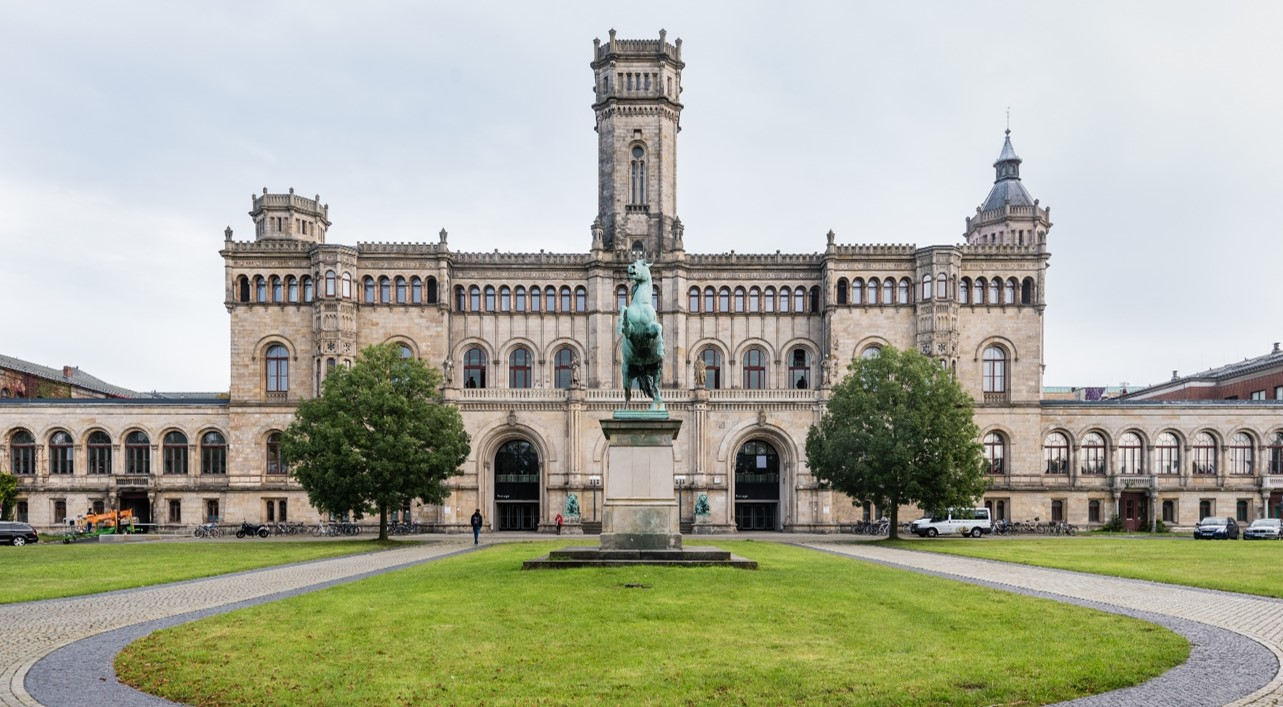
\includegraphics[width=0.65\textwidth]{figures/luh_default_presentation_title_image.jpg}}

% Title page: luhstyle
% \setbeamertemplate{title page}[luhstyle]
% % Add optional title image here
% \addtitlepageimage{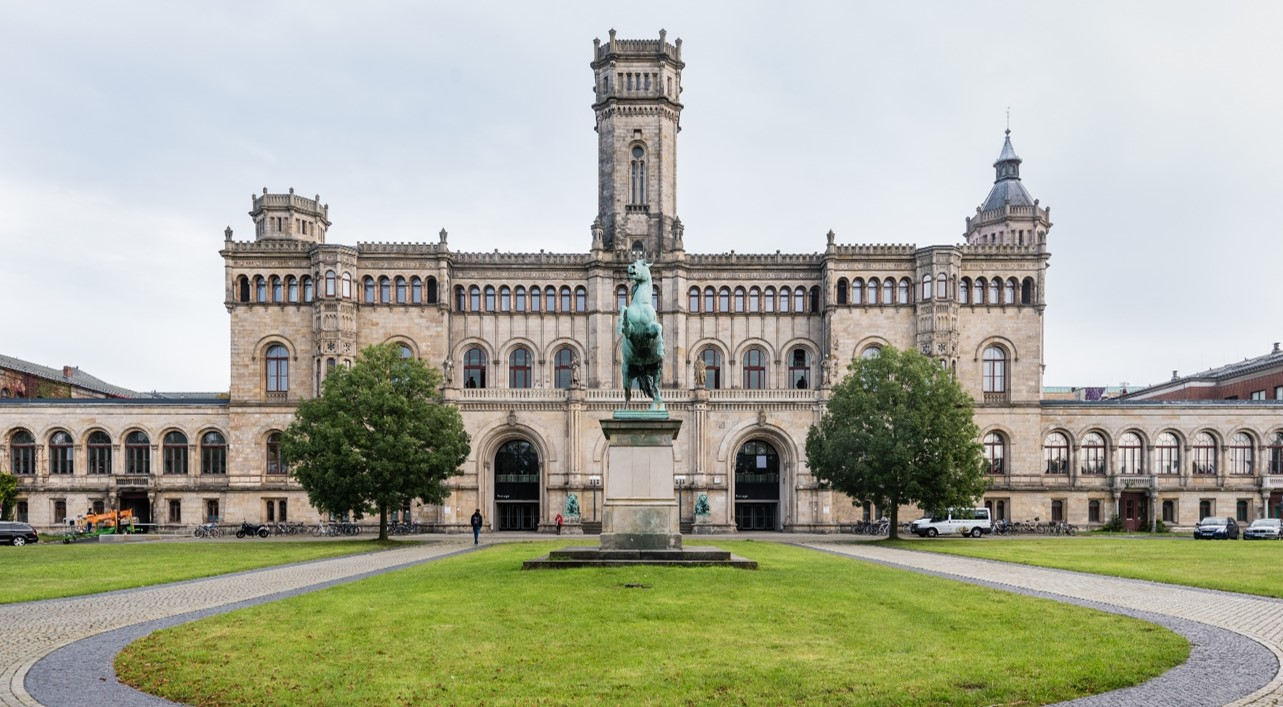
\includegraphics[width=0.75\textwidth]{figures/luh_default_presentation_title_image.jpg}}

\author[Abedjan \& Lindauer]{Ziawasch Abedjan \& Marius Lindauer\\[1em]
	
\includegraphics[height=\logoheight]{../latex_main/figures/luh_logo_rgb_0_80_155.pdf}\qquad
	
\includegraphics[height=\logoheight]{../latex_main/figures/DBIS_Kurzlogo.png}\qquad

\includegraphics[height=\logoheight]{../latex_main/figures/TNT_darkv4}\qquad

\includegraphics[height=\logoheight]{../latex_main/figures/L3S.jpg}	}
\date{Summer Term 2022; \hspace{0.5em} {
\includegraphics[height=1.5em]{../latex_main/figures/Cc-by-nc-sa_icon.svg.png}}; based on \href{https://ds100.org/fa21/}{[DS100]}
}


%%% Custom Packages
%----------------------------------------------------------------------
% Create dummy content
\usepackage{blindtext}

% Adds a frame with the current page layout. Just call \layout inside of a frame.
\usepackage{layout}


%%% Macros
%\renewcommand{\vec}[1]{\mathbf{#1}}
% \usepackage{bm}
%\let\vecb\bm

\title[Regression]{DS: Simple Linear Regression}
\subtitle{RMSE and Multiple R$^2$}

\graphicspath{ {./figure/} }
%\institute{}


\begin{document}
	
	\maketitle
	\begin{frame}{Evaluating models}
	    What are some ways to determine if our model was a good fit to our data?
	    \begin{itemize}
	        \item Look at MSE or RMSE.
	        \item Look at the correlations.
	        \item Look at a residual plot.
	        \begin{itemize}
	            \item Residuals are defined as being the difference between actual and predicted y values. 
	            \begin{itemize}
	                \item  $e_i = y_i - \hat{y}_i$
	            \end{itemize}
	        \end{itemize}
	    \end{itemize}
	\end{frame}
	
	
	\begin{frame}{Root Mean Squared Error (RMSE)}
	    \begin{equation*}
	        RMSE(y,\hat{y}) = \sqrt{\frac{1}{n}\sum\limits_{i=1}^n(y_i - \hat{y}_i)^2}
	    \end{equation*}
	    Root mean squared error is defined as being the square root of the mean squared difference between predictions and their true values.

	    \begin{itemize}
	        \item It is the square root of MSE, which is the average loss that we’ve been minimizing to determine optimal model parameters.
	        \item \alert{RMSE is in the same units as y}.
	        \item A lower RMSE indicates more “accurate” predictions.
	        \begin{itemize}
	            \item Lower average loss across the dataset.
	        \end{itemize}
	    \end{itemize}
	\end{frame}
	
	
	
	\begin{frame}{Comparing RMSEs}
	
	    \vspace{-2em}
	    \begin{columns}
	    
	        \begin{column}{.6\textwidth}
	        
	                \begin{itemize}
	                    \item For the constant model with squared loss, RMSE is  $\sigma_y$   
	                    \begin{itemize}
	                        \item MSE(sample mean) = sample variance.
	                        \item This is a good baseline to compare with.
	                    \end{itemize}
	                    \item Using just the data we trained our model on, it is impossible for RMSE to go up by adding features.
	                    \begin{itemize}
	                        \item If a new feature (e.g. “does a player like the color red?”) we’ve added doesn’t help lower average loss, its weight will just be set to 0.
	                        \item When we start evaluating models on unseen data, this is no longer true.
	                        \begin{itemize}
	                            \item We will see why in another lectures.
	                        \end{itemize}
	                    \end{itemize}
	                    \item Soon, we will look at “training error” and “testing error”. The errors that we look at are RMSEs.
	                \end{itemize}
	        \end{column}
	            
	        \begin{column}{.4\textwidth}
	        
	                \begin{equation*}
	                 RMSE(y,\hat{y}) = \sqrt{\frac{1}{n}\sum\limits_{i=1}^n(y_i - \hat{y}_i)^2}
	            \end{equation*}
	            prediction PTS = 3.98 + 2.4 $\cdot$ AST

	                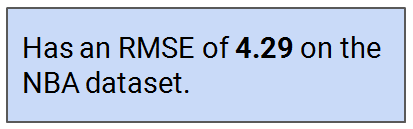
\includegraphics[scale=.3]{Bild11}
	            
	            prediction PTS = 2.163 + 1.64 $\cdot$ AST + 1.26 $\cdot$ 3PA

	                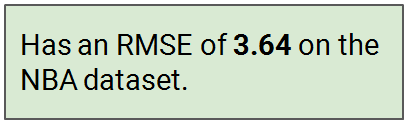
\includegraphics[scale=.3]{Bild12}

	        \end{column}
	    \end{columns}
	\end{frame}
	
	
	
	\begin{frame}{Multiple R²}
	
	    When we had just one feature $x$, we were able to look at the correlation coefficient $r$ to get a sense of how strong the linear association between x and y was. 
	    
	    \begin{itemize}
	        \item The further $r$ was from 0, the stronger the linear association between $x$ and $y$.
	        \begin{itemize}
	            \item Looking at $r$ alone isn’t enough. 
	        \end{itemize}
	        \item Here we have multiple features. We could (and sometimes do!) look at the correlation between each feature and our true y values individually.
	        \item However, we are also interested in measuring the strength of the linear association between our actual y and predicted y.
	        \begin{itemize}
	            \item We want this relationship to be as close to the line y = x as possible.
	        \end{itemize}
	    \end{itemize}
	    
	        \centering
	        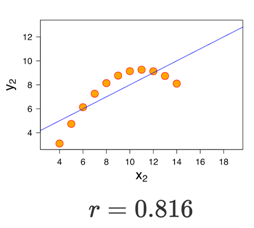
\includegraphics[scale=.4]{Bild13}
	   
	\end{frame}
	
	
	\begin{frame}{Multiple R²}
	   We define the multiple R² value as the square of the correlation between the true $y$ and predicted $y$. This is also referred to as the coefficient of determination.
	    \begin{equation*}
	        R^2 = [r(y,\hat{y})]^2
	    \end{equation*}
	    Since it is the square of a correlation coefficient (which ranged between -1 and 1), R² ranges between 0 and 1. Another way of expressing R², in linear models that have an intercept term, is
        \begin{equation*}
	        R^2 = \frac{\text{variance of fitted values}}{\text{variance of y}} = \frac{\sigma_{\hat{y}}^2}{\sigma_{y}^2}
	    \end{equation*}
	   Thus, we can interpret R² as the proportion of variance in our true $y$ that our fitted values (predictions) capture, or “the proportion of variance that the model explains.”
	\end{frame}
	
	
	
	
	\begin{frame}{Multiple R²}
	    \begin{columns}
	        \begin{column}{.6\textwidth}
	                \begin{itemize}
	                    \item As we add more features, our fitted values tend to become closer and closer to our actual y values. Thus, R² increases.
	                    \begin{itemize}
	                        \item The simple model (AST only) explains 45.7\% of the variance in the true y.
	                        \item The AST & 3PA model explains 60.9\%.
	                    \end{itemize}
	                    \item Adding more features doesn’t always mean our model is better, though!
	                    \begin{itemize}
	                        \item We are a few lectures away from understanding why.  
	                        \item “Adjusted R²” accounts for this.
	                    \end{itemize}
	                \end{itemize}
	        \end{column}
	            
	        \begin{column}{.4\textwidth}
	        \vspace{-1em}
	                \begin{equation*}
	                     R^2 = \frac{\text{variance of fitted values}}{\text{variance of y}}
	                 \end{equation*}
	            prediction PTS = 3.98 + 2.4 $\cdot$ AST
	            \begin{figure}
	                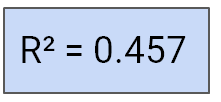
\includegraphics[scale=.4]{Bild14}
	            \end{figure}
	            
	            prediction PTS = 2.163 + 1.64 $\cdot$ AST + 1.26 $\cdot$ 3PA
	             \begin{figure}
	                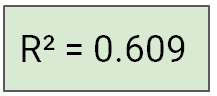
\includegraphics[scale=.4]{Bild15}
	            \end{figure}
	        \end{column}
	    \end{columns}
	\end{frame}
\end{document}